\documentclass{sigchi}

% Use this command to override the default ACM copyright statement (e.g. for preprints). 
% Consult the conference website for the camera-ready copyright statement.


%% EXAMPLE BEGIN -- HOW TO OVERRIDE THE DEFAULT COPYRIGHT STRIP -- (July 22, 2013 - Paul Baumann)
% \toappear{Permission to make digital or hard copies of all or part of this work for personal or classroom use is 	granted without fee provided that copies are not made or distributed for profit or commercial advantage and that copies bear this notice and the full citation on the first page. Copyrights for components of this work owned by others than ACM must be honored. Abstracting with credit is permitted. To copy otherwise, or republish, to post on servers or to redistribute to lists, requires prior specific permission and/or a fee. Request permissions from permissions@acm.org. \\
% {\emph{CHI'14}}, April 26--May 1, 2014, Toronto, Canada. \\
% Copyright \copyright~2014 ACM ISBN/14/04...\$15.00. \\
% DOI string from ACM form confirmation}
%% EXAMPLE END -- HOW TO OVERRIDE THE DEFAULT COPYRIGHT STRIP -- (July 22, 2013 - Paul Baumann)


% Arabic page numbers for submission. 
% Remove this line to eliminate page numbers for the camera ready copy
% \pagenumbering{arabic}


% Load basic packages
\usepackage{balance}  % to better equalize the last page
\usepackage{graphics} % for EPS, load graphicx instead
\usepackage{times}    % comment if you want LaTeX's default font
\usepackage{url}      % llt: nicely formatted URLs
\usepackage{subcaption}
\usepackage{float}
% llt: Define a global style for URLs, rather that the default one
\makeatletter
\def\url@leostyle{%
  \@ifundefined{selectfont}{\def\UrlFont{\sf}}{\def\UrlFont{\small\bf\ttfamily}}}
\makeatother
\urlstyle{leo}


% To make various LaTeX processors do the right thing with page size.
\def\pprw{8.5in}
\def\pprh{11in}
\special{papersize=\pprw,\pprh}
\setlength{\paperwidth}{\pprw}
\setlength{\paperheight}{\pprh}
\setlength{\pdfpagewidth}{\pprw}
\setlength{\pdfpageheight}{\pprh}

% Make sure hyperref comes last of your loaded packages, 
% to give it a fighting chance of not being over-written, 
% since its job is to redefine many LaTeX commands.
\usepackage[pdftex]{hyperref}
\hypersetup{
pdftitle={SIGCHI Conference Proceedings Format},
pdfauthor={LaTeX},
pdfkeywords={HCI, Cooperative, Spaceship, Game},
bookmarksnumbered,
pdfstartview={FitH},
colorlinks,
citecolor=black,
filecolor=black,
linkcolor=black,
urlcolor=black,
breaklinks=true,
}

% create a shortcut to typeset table headings
\newcommand\tabhead[1]{\small\textbf{#1}}


% End of preamble. Here it comes the document.
\begin{document}

\title{SpaceRescue: A communicative Game for Interactive Floors}

\numberofauthors{1}
\author{
  \alignauthor Daniel Birnstiel, Patrick Kuhn, Fabian Paul, Lennard Wolf\\
      \medskip
    \affaddr{Hasso Plattner Institute}\\
    \affaddr{Prof.-Dr.-Helmert-Str. 2-3}\\
    \affaddr{14482 Potsdam, Germany}\\
    \email{$ \{ $ daniel.birnstiel, patrick.kuhn, fabian.paul, lennard.wolf $ \} $@student.hpi.de }\\
}

\maketitle

\begin{abstract}
\vspace{1mm}
After looking upon the possibilities of interactive floors and taking into account the immense demand for video games today, we developed \textit{SpaceRescue}. \textit{SpaceRescue} is designed as a fun prototype for communicative, interactive floor based games and demonstrates, how playing games at home can once again involve moving the entire body
again - and not just your thumbs.


The two to three players' goal is the joint reaching of levels by performing tasks that are randomly given to each player. These tasks can then be carried out by the player himself or he can tell his partners to do it for him since they are closer to the task-subject. 

\end{abstract}

\keywords{
	SpaceRescue; Communication; Interactive Floors; Body Movement
}

\section{Introduction}
\vspace{1mm}
With the advent of the \textit{Internet of Things} and thus the rising digital Interaction with everything around us, floors will soon become intelligent entities just like our phones are today. 

But next to all the productive things we can now do with our devices, we also want to integrate them into our leisure time. Just like touch screens revolutionised the way we play games, interactive floors will again push the boundaries of the way we think about enjoying ourselves through games.

To understand what players want from a game, we interviewed J\"org Friedrich, a professional Game Designer at AAA Game Development Studio \textit{Yager}, Willy Scheibel, a Game Development Lecturer at \textit{HPI}, as well as Theresa Zobel, a representative of our target group, the casual gamer. From these interviews we learned that:
\begin{itemize}
\item The Game mechanics are the very most important part in the success of a game and should mostly be based on already proven concepts.
\item Today's players have a low attention span and thus want to understand the game right away.
\item Gamers always want to be challenged but not to the point where they get frustrated.
\item Next to the challenge, gamers also need a purpose for their actions. This might involve a story or the immersion in a virtual world.
\item Pleasing graphics are nice to have but not overly important, especially not photorealism.
\item Most Gamers today like to play Cooperative Games rather than Single Player Titles.
\end{itemize}


This is why we started out contemplating different mini games and at some point even considered creating a mini game collection. But what we saw as the main advantage of an interactive floor based game was the fact that the player might not be alone, but rather be in the same room with others and cooperate. 

This is why we chose to concentrate on three main goals for our project: \textbf{Communication}, \textbf{Cooperation} and \textbf{Discoverability}.



\begin{figure}[!h]
\centering
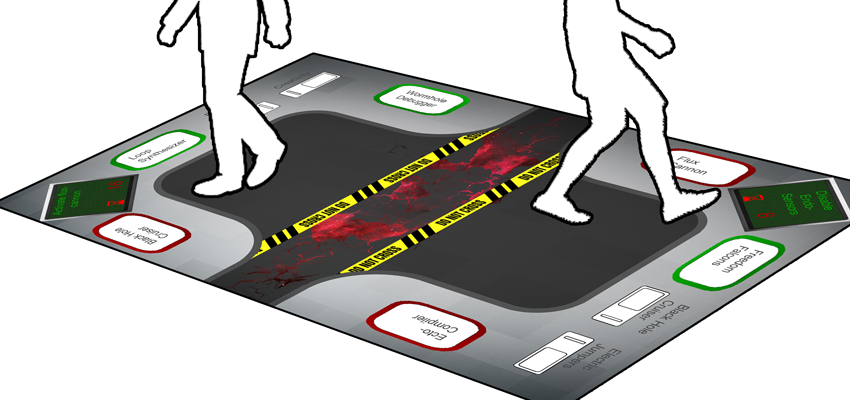
\includegraphics[width=0.99\columnwidth]{walkthrough/totale2}
\caption{The Game in action.}
\label{fig:figure1}
\end{figure}
\pagebreak




\section{The Concept of the Game}
\vspace{1mm}
The game is set on a spaceship, which is on the edge of destruction and the players on earth are the astronauts to save the ship. They have to get on the beaming platforms to beam onto the spaceship, where they get their tasks. These tasks involve flipping switches and pressing buttons, which make up the control bridge of the ship. 

Since these widgets are not always close to the player who got a new task, he will often have to tell his partner(s) to do it for him instead. But a task is only active for a limited amount of time and if a task is not performed in time, it's game over. \newline
After a certain number of tasks the players will get to a new and harder level where all controls will change and the game goes on. Winning as such is \textit{not} possible, the motivation is rather staying alive for as long as possible.
\section{Walkthrough}
\vspace{1mm}
In our sample scenario two users A and B want to play a game of \textit{Cooperative Spaceship Rescue} with the goal to reach the second Level. As the users enter the floor, they will start out in the \textit{Beaming Area}, as shown in Figure 8.

\subsection{The Beaming Area}
\vspace{3mm}

\begin{figure}[h]
\centering
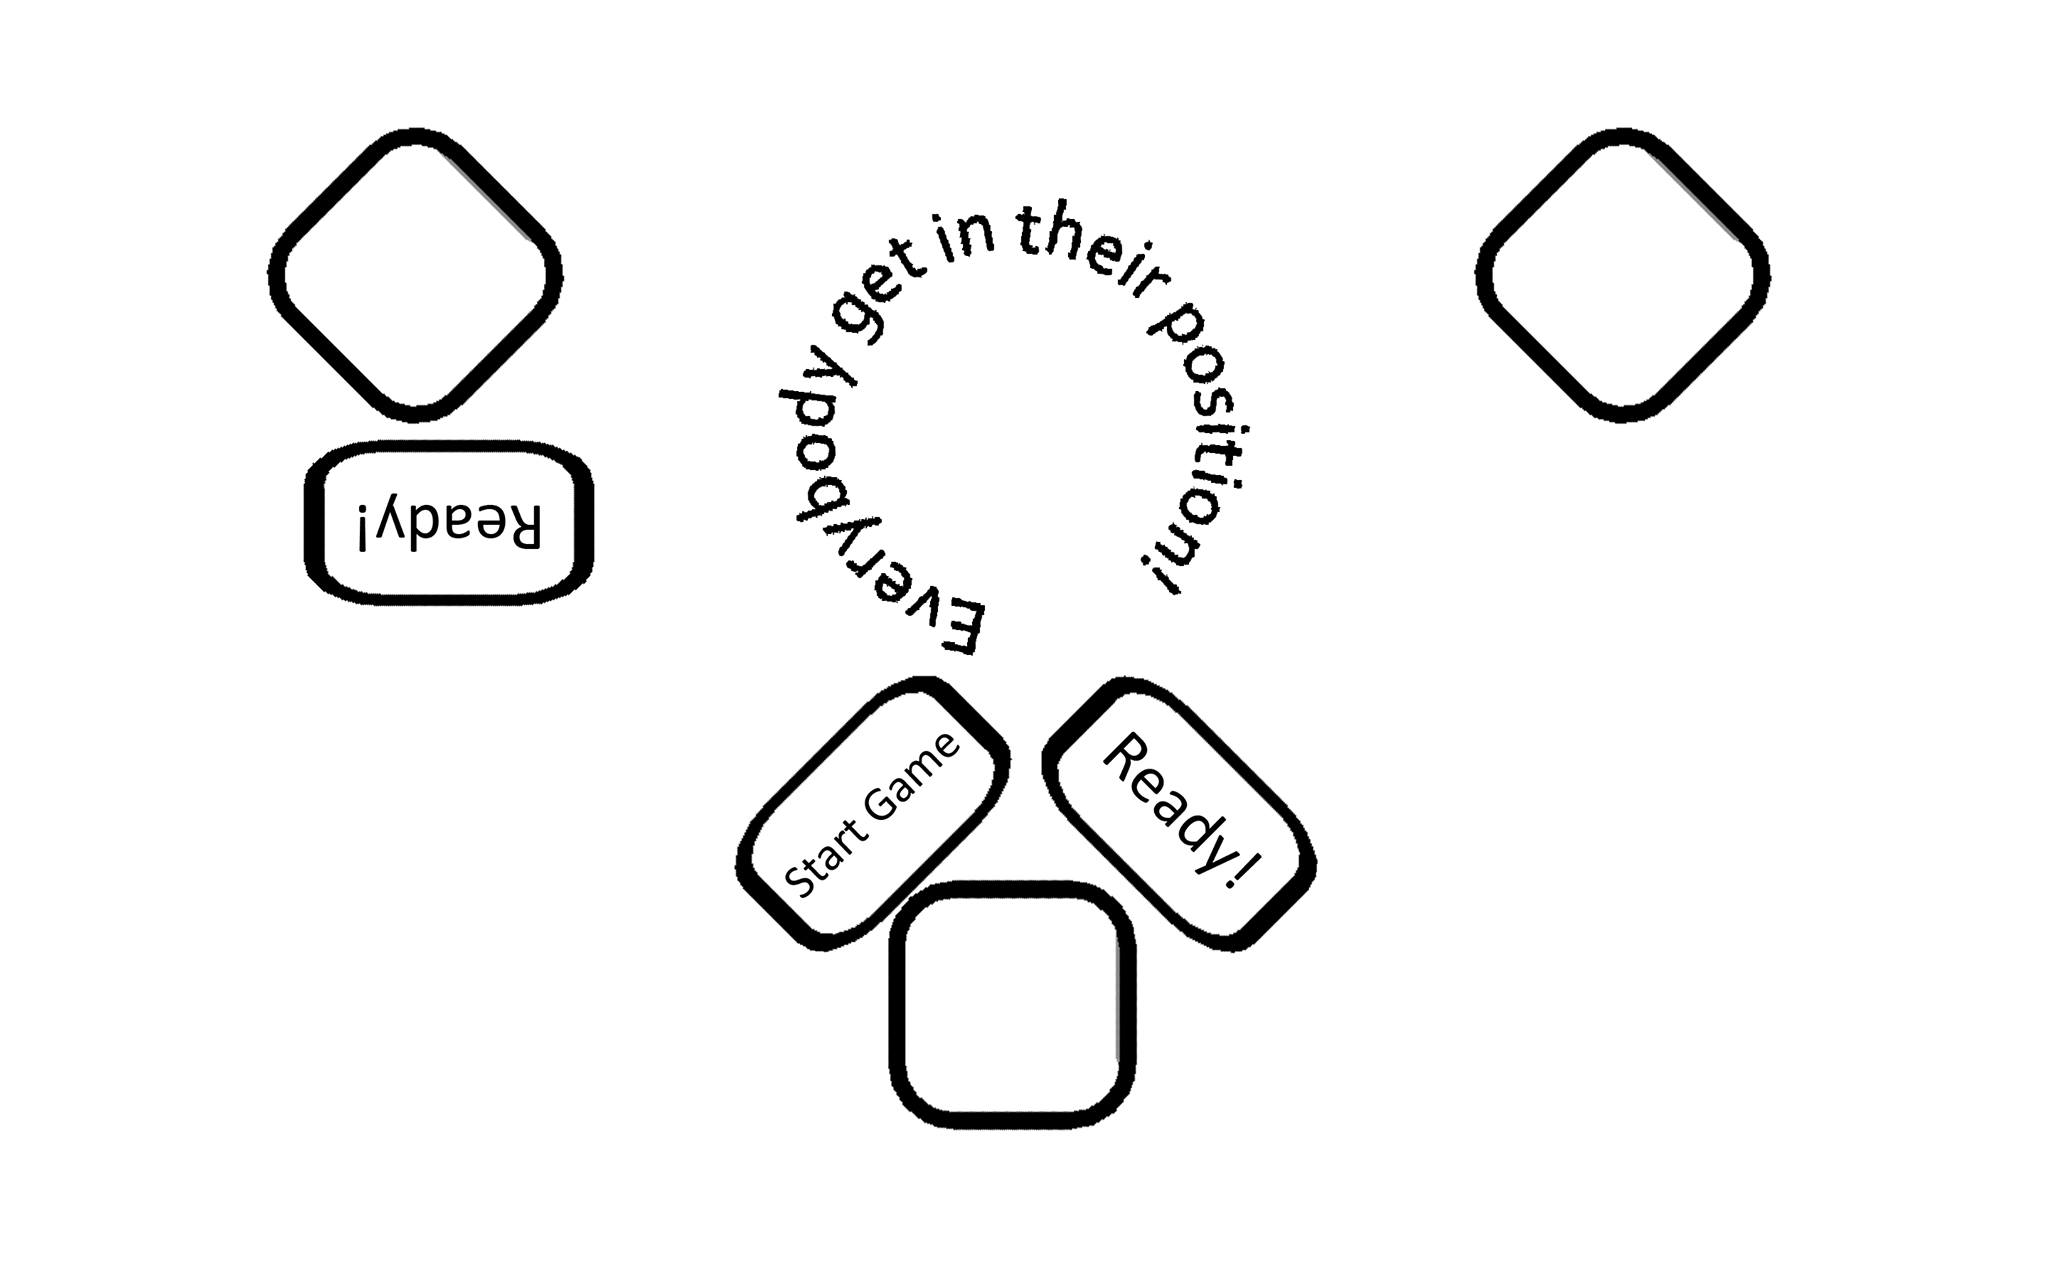
\includegraphics[width=0.8\columnwidth]{beamingArea}
\caption{The Beaming Area from the bird's perspective.}
\label{fig:beamingArea}
\end{figure}



\begin{enumerate}
\item Users walk to the \textit{Beaming platforms} and want to start our game.
\item To start the game they have to enter one the circle while the label in mid is rotating \textit{Ready?}-Buttons appear and will change the to a \textit{Ready!} after tapping on them.
\begin{figure}[H]
\centering
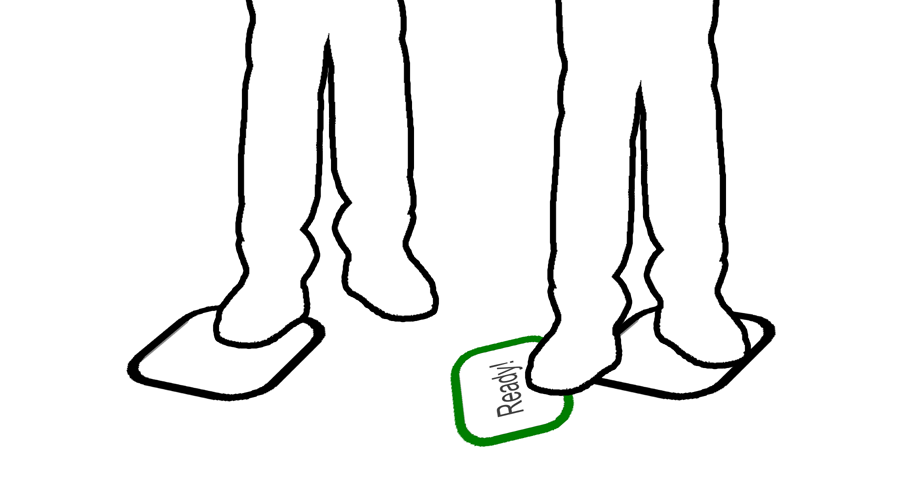
\includegraphics[width=0.9\columnwidth]{walkthrough/klein/beamingarea1+2a}
\caption{Steps 1 and 2a}
\label{fig:gamingArea}
\end{figure}

\item The first player to step on a \textit{Beaming platform} gets a \textit{Start Game}-Button when everybody has tapped on their \textit{Ready?}-Button.
\item That player can now start the Game by tapping on the \textit{Start Game}-Button. After it the screen will change to our \textit{Gaming Area}.
\end{enumerate}

\begin{figure}[H]
\centering
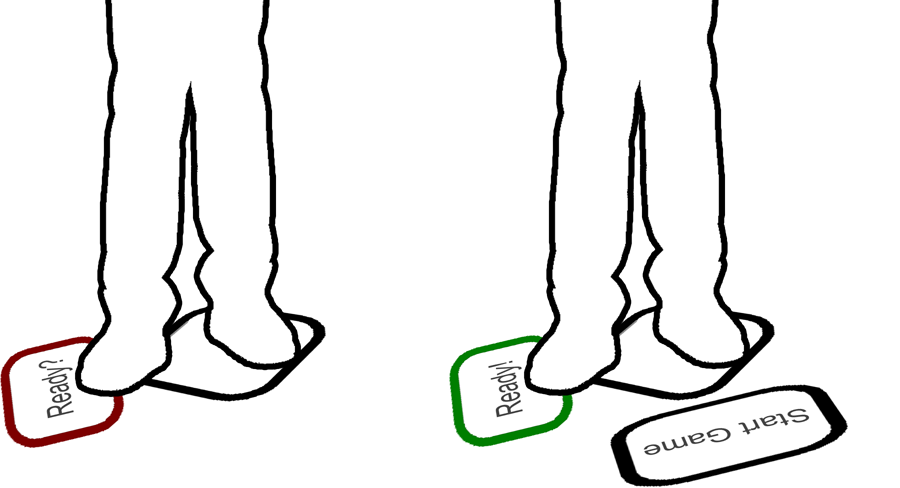
\includegraphics[width=0.9\columnwidth]{walkthrough/klein/beamingarea2b+3}
\caption{Steps 2b and 3}
\label{fig:gamingArea}
\end{figure}




\subsection{The Gaming Area}



\begin{figure}[H]
\centering
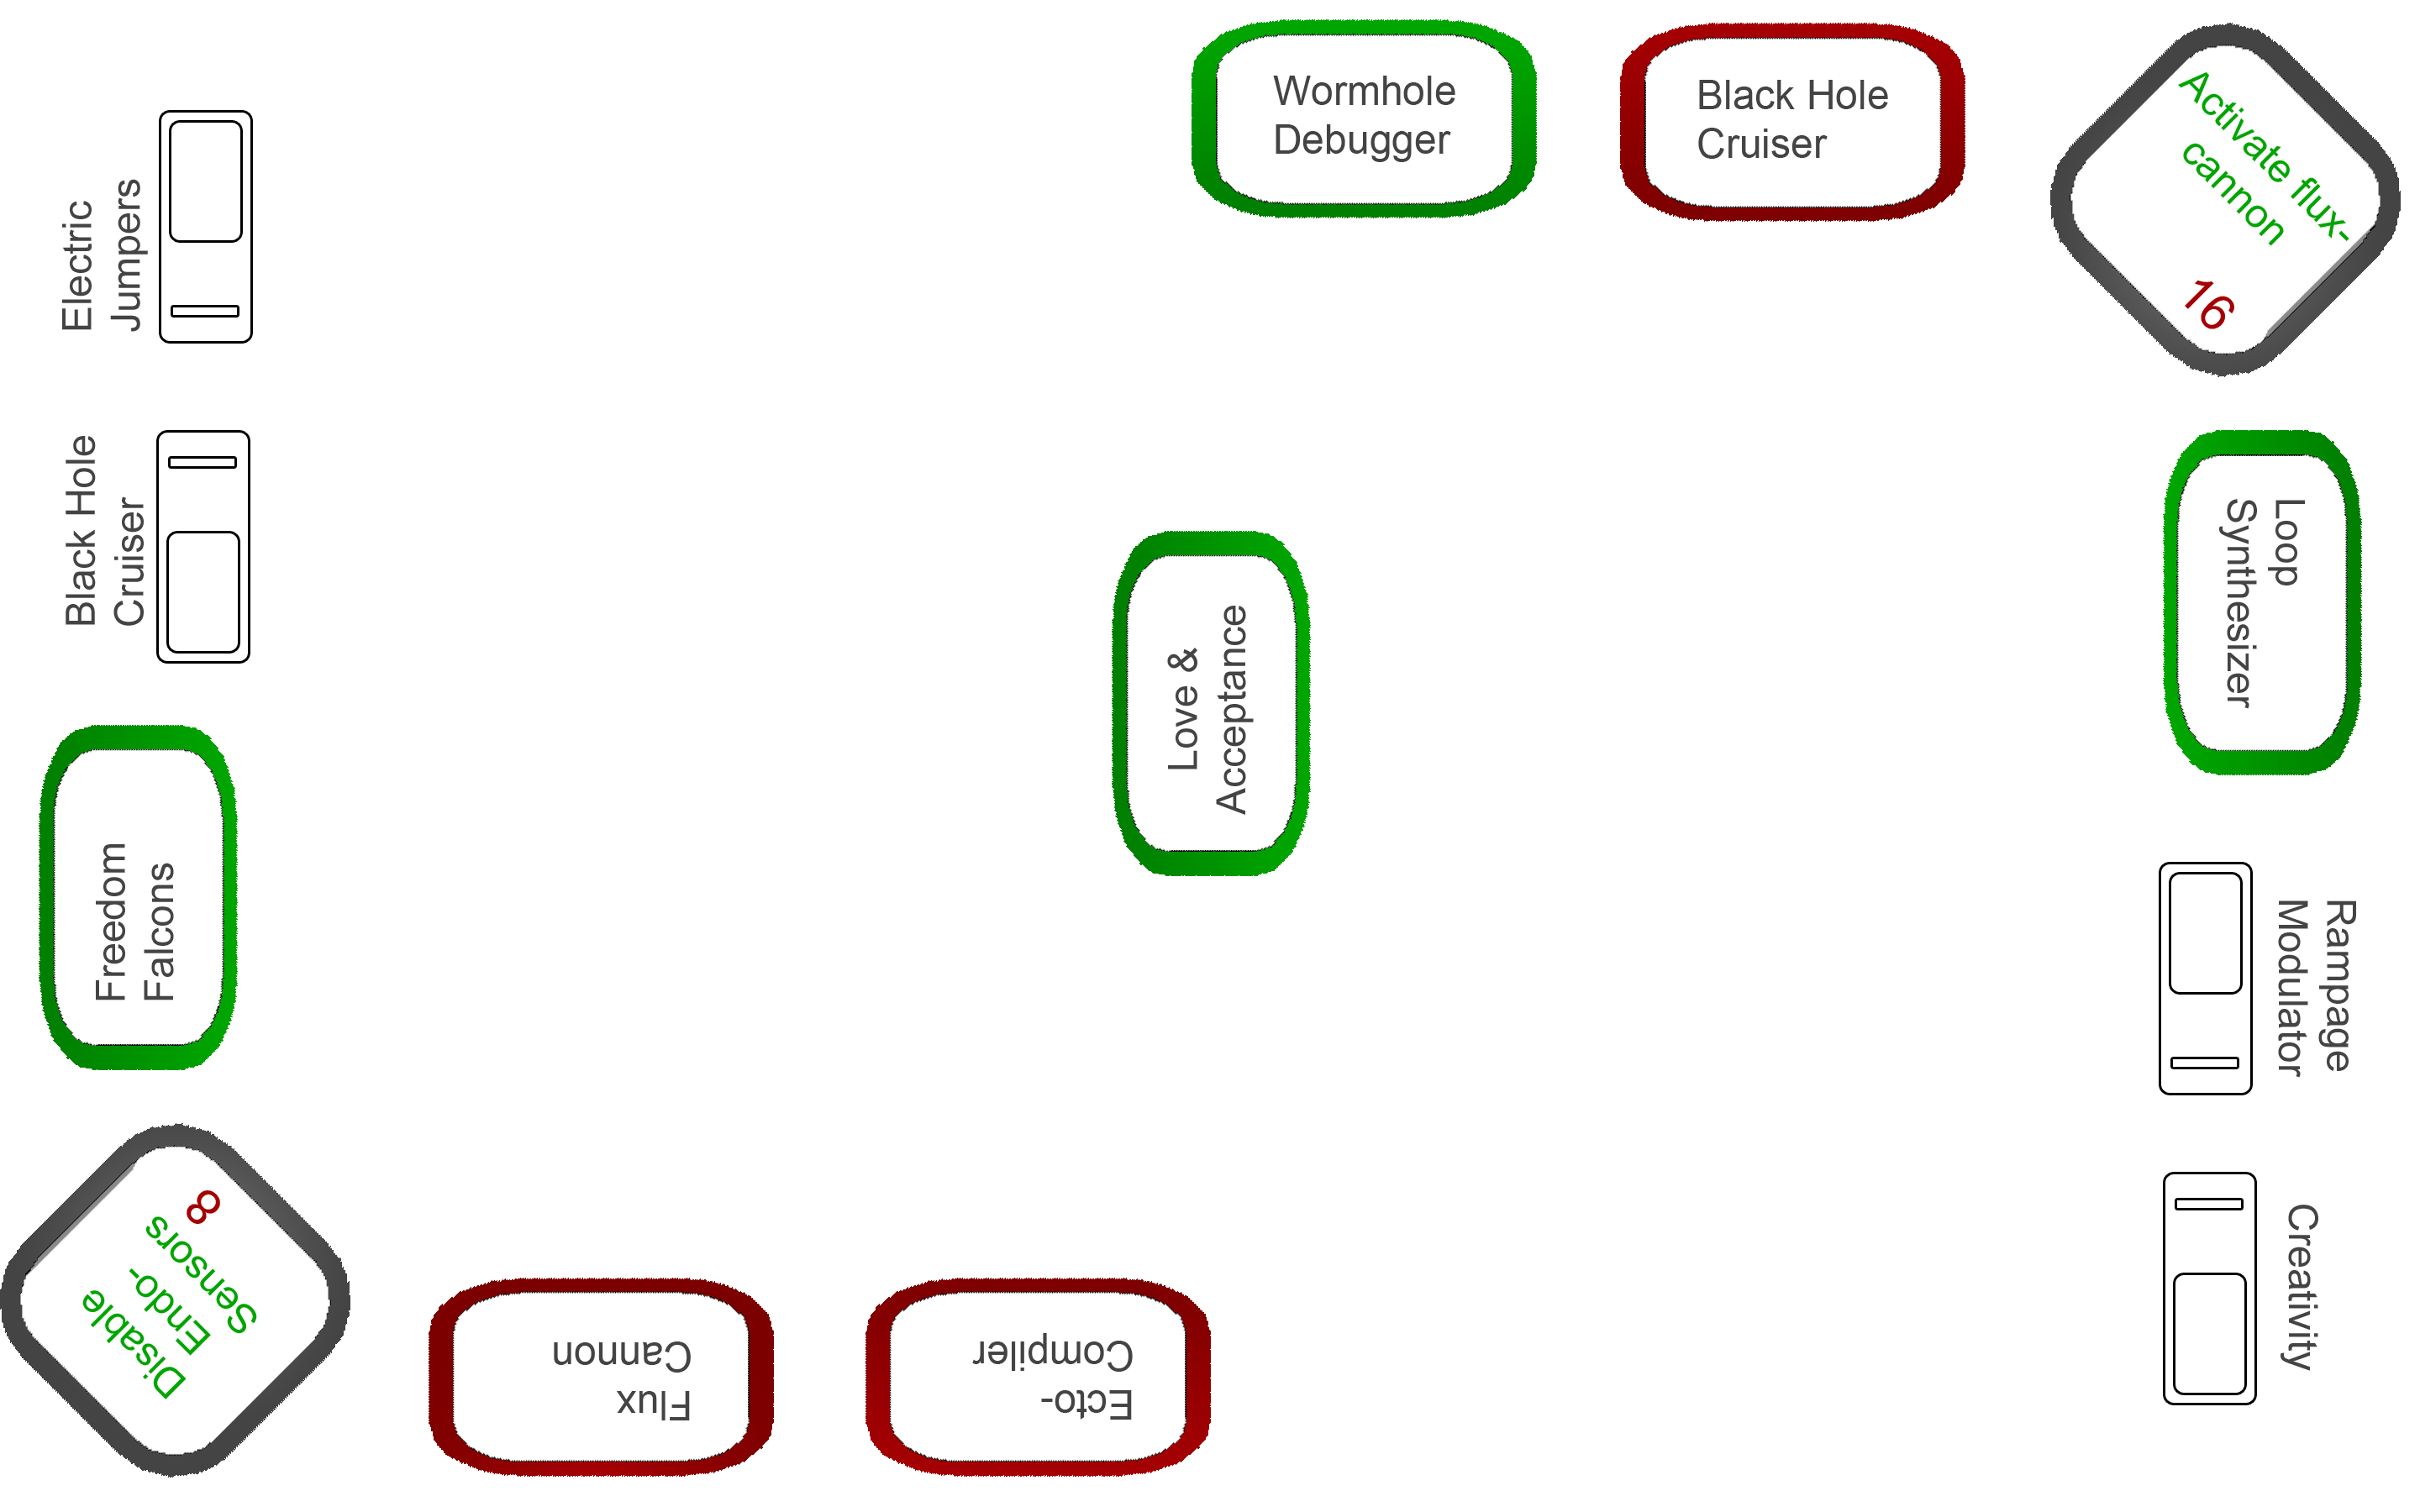
\includegraphics[width=0.9\columnwidth]{walkthrough/gamingarea}
\caption{The Gaming Area from the bird's perspective.}
\label{fig:beamingArea}
\end{figure}
\vspace{2mm}
\begin{enumerate}
\item Players A and B mention the two highlighted task panels behind them and turn around.
\item There, each player reads his instructions and sees their timer counting down.


\begin{figure}[H]
\centering
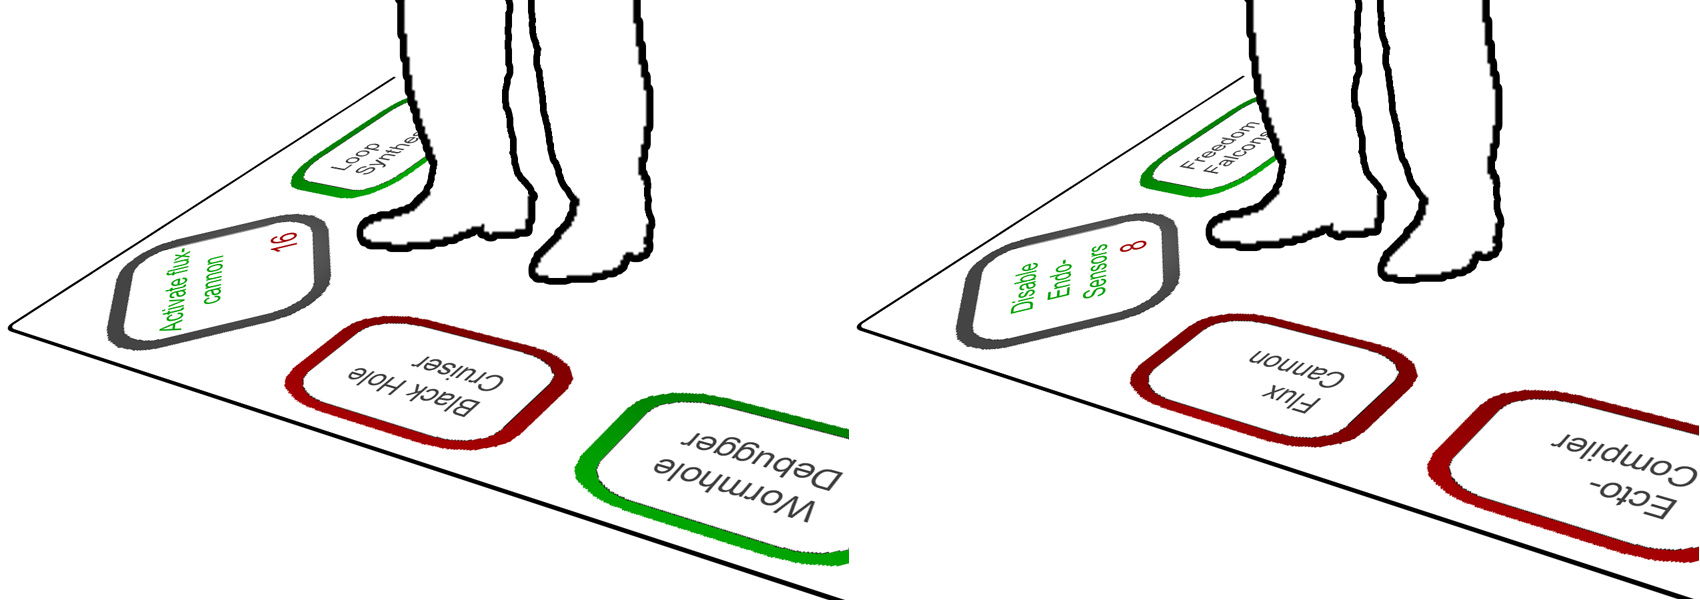
\includegraphics[width=0.99\columnwidth]{walkthrough/klein/gamingarea3+4}
\caption{Steps 3 and 4}
\label{fig:gamingArea}
\end{figure}

\item Player A gets task X (for example "Activate Flux Cannon" as shown in Figure 6).
\item Player B gets task Y (for example "Disable Endo-Sensors" as shown in Figure 6).
\item A and B try to perform their task by communicating or finding their widget.
\item After a task has been performed before the corresponding timer has counted to zero, a new task is be generated and the timer is reset.

\begin{figure}[H]
\centering
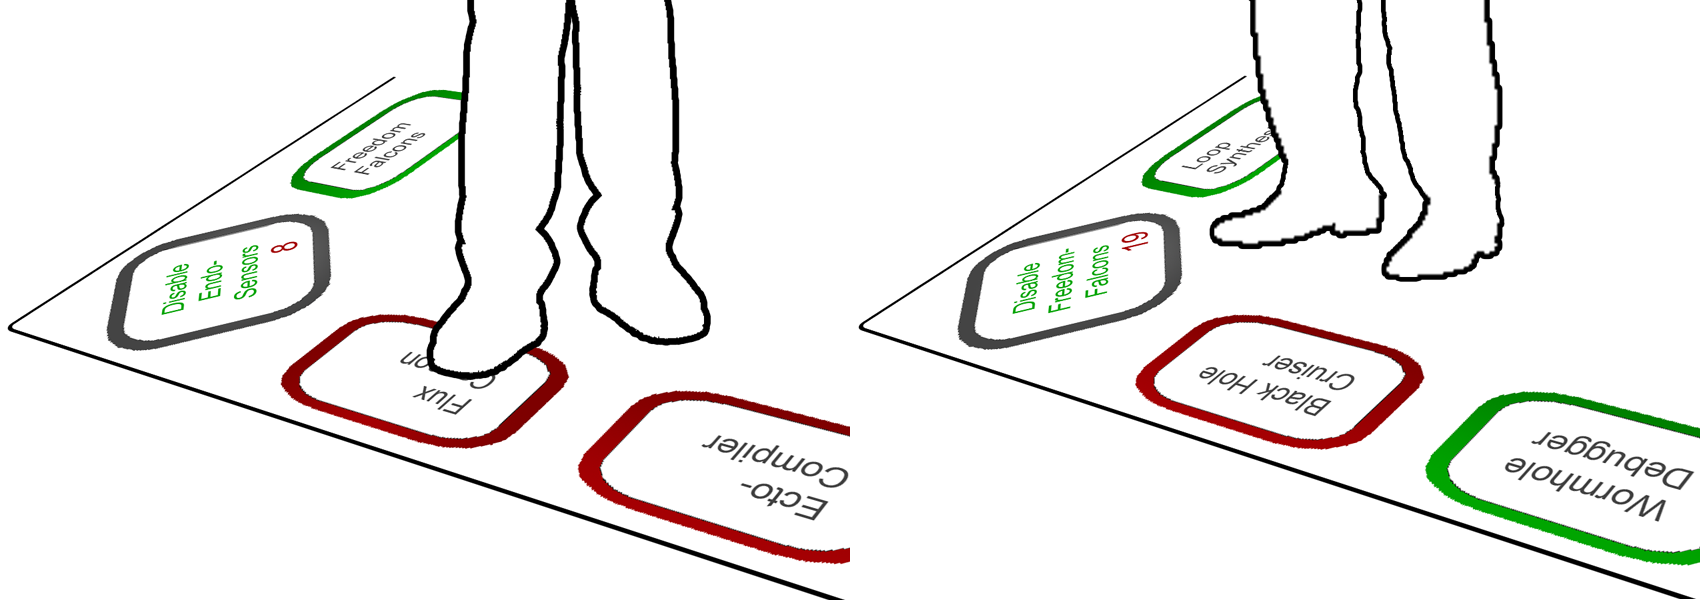
\includegraphics[width=0.99\columnwidth]{walkthrough/klein/gamingarea5+6}
\caption{Steps 5 and 6}
\label{fig:gamingArea}
\end{figure}
\item Repeat steps 3. to 6. until a new Level is generated and the players have reached their goal.
\end{enumerate}


\section{Design}
\vspace{1mm}
In this section we will discuss the design choices we made to achieve our goals for \textbf{Communication}, \textbf{Cooperation} and \textbf{Discoverability}.

\subsection{Cooperation as a Paradigm}
\vspace{1mm}
Our first idea was to create an application which would consist of various \textit{minigames}, which could be successively played against each other. The problem with this approach was, as Willy Scheibel pointed out in our contextual inquiry, that this approach would only allow users to interact with each other to certain degree. Playing by taking turns would not actually require the other player to be there, thus the whole concept of being together in a room vanishes. 

Therefore we wanted to integrate cooperation as a paradigm for our game design by creating goals which would have to be performed by \textit{both} users. Furthermore we use the spatial distribution of our tasks-subjects to encourage interaction between the players, rather than having them only perform their own tasks. 
 
\subsection{Standing in a defined Area as Login Mechanism}
\vspace{1mm}
Initially we thought about having the users register to the system with an on-floor keyboard and then log in every time they enter the floor. During paper prototyping we encountered that it is really tedious for the user to type in his name, since tapping on small buttons requires precision and having the buttons spread makes them hard to use because it would be necessary to walk over them to get to the destination. 

We decided to create areas in which the users have to stand to start the game. The paper prototyping and the heuristic evaluation showed that this was easily understandable, especially because of the conceptual model of the \textit{beaming area} of spaceships from \textit{Star Trek}. 

\begin{figure}[H]
\centering
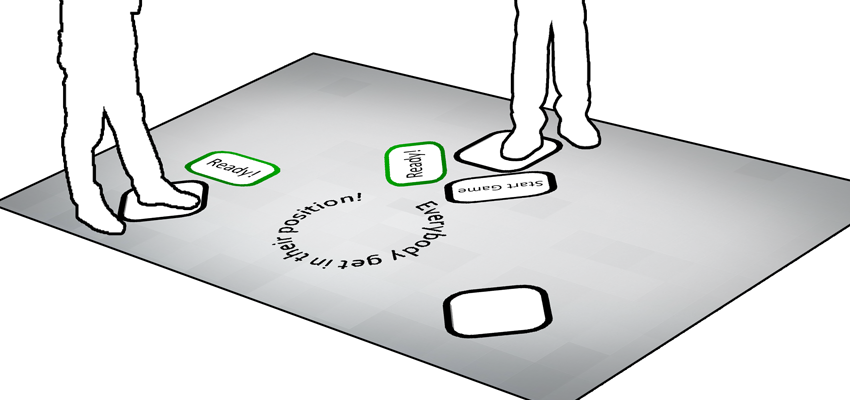
\includegraphics[width=0.99\columnwidth]{walkthrough/totale1}
\caption{Two users logging in through the \textit{Beaming Platforms}}
\label{fig:beamingArea}
\end{figure}


\subsection{Avoiding roles as a Game Mechanic}
\vspace{1mm}
Originally we came up with the idea of having different roles for each user, so that each would only be able to carry out certain tasks. As an example, the role of the \textit{captain} was assigned to the first person entering a beaming platform. That user was then the one able to start the game and they would also have special rights to certain widgets and so on. In our paper prototyping process, most of the testers asked about the meaning of those roles and having to explain it to them in more than a sentence showed how this concept was hardly discoverable and would just \textit{mode the user in}.

For these reasons we replaced the concept of roles with more specific tasks.

\subsection{Explaining System Status with Conceptual Models}
\vspace{1mm}
As we started designing our game, we used menus and text fields to let the user start a game or change a level. This approach seemed to work out quite well in paper prototyping, since the change of level for example would require some time to reconstruct the floor anyway. But as we started testing our application on the floor the change of status, especially the switching between two levels did not appear natural. 

As a result we added areas with a ladder texture to explain the switch to the next level. Moreover we use beaming platforms as login mechanism instead of a introduction dialog to have a consistent appearence in our whole game (hier will ich sagen, dass wir alles was der User sieht durch unsere Welt erklären statt durch Dialoge; wenn jemandem ne bessere Formulierung einfällt gerne austauschen)

\subsection{Having a distinct Exit Button}
\vspace{1mm}
When we faced the issue of how the game should be terminated, our initial solution was to just let the users walk off the floor and wait until the timer would run out. But during the heuristic evaluation, almost all of our testers asked us how they could end the game. This showed us that having no visual representation to use some functionality of the system is not at all discoverable. 

To solve this problem we introduced a distinct exit button, which can be pressed to ensure a controlled ending of the game. This is important because now the user has full control over the system at any time. 

\section{Conclusion}
\vspace{1mm}

Creating a game for a completely new Platform turned out to be a bigger challenge than first anticipated, since most classic gaming concepts were not applicable anymore. But talking to both gamers and the professionals in the field gave us great insights into what makes a good game. These insights made us create \textit{Cooperative Spaceship Rescue}, a game that we think of as really showing the possibilities for communication and involving of the whole body in Interactive Floor based games. \newline


\textit{Cooperative Spaceship Rescue} may not be a perfectly rounded, market-ready game, but can rather be seen as a fun prototype demonstrating the aforementioned possibilities.


\balance


\end{document}
